\documentclass[12pt]{article}

\usepackage{tikz}
\usetikzlibrary{arrows,shapes.gates.logic.US,shapes.gates.logic.IEC,calc}
\usepackage{listings}
\usepackage{graphics}
\usepackage{graphicx}
\usepackage{amsmath, amssymb}
\usepackage{./karnaugh-map}
\usepackage{xcolor}
\usepackage{color}
\usepackage[margin=1in,footskip=.25in]{geometry}

\definecolor{dkgreen}{rgb}{0,0.6,0}
\definecolor{gray}{rgb}{0.5,0.5,0.5}
\definecolor{mauve}{rgb}{0.58,0,0.82}
 
\definecolor{codegreen}{rgb}{0,0.6,0}
\definecolor{codegray}{rgb}{0.5,0.5,0.5}
\definecolor{codepurple}{rgb}{0.58,0,0.82}
\definecolor{backcolour}{rgb}{0.95,0.95,0.92}
 
\lstdefinestyle{mystyle}{
    backgroundcolor=\color{backcolour},   
    commentstyle=\color{codegreen},
    keywordstyle=\color{magenta},
    numberstyle=\ttfamily\footnotesize\tiny\color{codegray},
    stringstyle=\color{codepurple},
    basicstyle=\ttfamily\footnotesize,
    breakatwhitespace=false,         
    breaklines=true,                 
    captionpos=b,                    
    keepspaces=true,                 
    numbers=left,                    
    numbersep=5pt,                  
    showspaces=false,                
    showstringspaces=false,
    showtabs=false,                  
    tabsize=3
}

\usepackage{xepersian}
\settextfont[Scale=1]{Vazir}

\begin{document}

\title{\large Hazard چیست و چگونه می توان مشکل Hazard را حل کرد ؟}

\maketitle

\lstset{style=mystyle}

hazard وقتی اتفاق می افتد که مسیر های مختلف ورودی به خروجی تاخیرهای زمانی مختلفی داشته باشند که باعث می شود خروجی صحیح در همه ی لحظه ها را نداشته باشیم\newline

3 نوع hazard در مدارهای دیجیتال وجود دارد :

\begin{enumerate}
	\item Static-Hazard
	\item Dynamic-Hazard
	\item Functional-Hazard
\end{enumerate}


\section{Static-Hazard}

static-hazard وقتی اتفاق می افتد که تغییر در ورودی باعث تنها یکبار تغییر لحظه ای در خروجی شود قبل از اینکه خروجی به مقدار نهایی  و اولیه اش تثبیت شود\newline

2 نوع static-hazard وجود دارد :

\subsection{static-1-hazard}

اگر خروجی در حالت 1 منطقی باشد و بعد از تغییر ورودی، خروجی به صورت لحظه ای به 0 برود و سپس دوباره به حالت 1 تثبیت شود می گوییم
static-1-hazard
 رخ داده است


\subsection{static-0-hazard}

اگر خروجی در حالت 0 منطقی باشد و بعد از تغییر ورودی، خروجی به صورت لحظه ای به 1 برود و سپس دوباره به حالت 0 ثابت شود می گوییم static-0-hazard رخ داده است


\begin{center}
	\includegraphics[scale=0.8]{./Static-hazards-1.jpg}
	%\caption{}
\end{center}

\section{تشخیص static-hazard با استفاده از نقشه ی کارنو}


برای تشخیص static-1-hazard مراحل زیر را طی می کنیم :

\begin{enumerate}
	\item تابع خروجی مدار را می نویسیم
	\item نقشه ی کارنو برای تابع خروجی را رسم می کنیم
	\item اگر هر زوج همسایه ی 1 ای وجود داشت که در تابع اصلی در نظر گرفته نشده بود، نشان دهنده وجود static-1-hazard می باشد
	
\end{enumerate}



مثال زیر را در نظر بگیرید :

\begin{center}
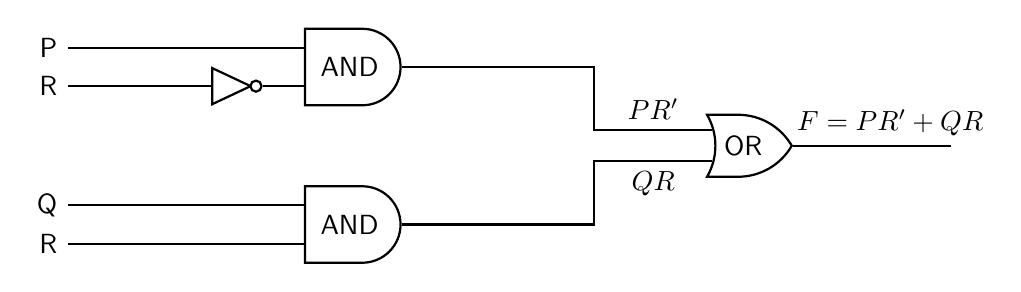
\begin{tikzpicture}[
        %Environment config
        font=\sffamily,
        thick,
        %Environment styles
        GateCfg/.style={
            logic gate inputs={normal,normal,normal},
            draw,
            scale=1
        }
    ]
    \path
        (0,0) node[and gate US,GateCfg](AND1){AND} 
            ++ (0,-2) node[and gate US,GateCfg](AND2){AND} 
            ++ (5,1) node[or gate US,GateCfg](OR1){OR}
        (AND1.input 3)
            ++ (-1,0) node[not gate US, draw](N1){};

    \draw
        (OR1.input 1) -- ++(-1.5,0)node [midway,anchor=south]{$PR^{\prime}$} |- (AND1.output) 
        
        (OR1.input 3) -- ++(-1.5,0)node [midway,anchor=north]{$QR$} |- (AND2.output)
        
        %(N2.output)--(AND2.input 3)
        
        (N1.output)--(AND1.input 3)
        
        %(N3.output)--(AND2.input 1)
        
        (AND1.input 1) 
            -- ++(-3,0) coordinate (init) node[anchor=east]{P}
            node[pos=0.6](temp){}
            
	  (AND2.input 1)
	  -- ++(-3,0) coordinate (init) node[anchor=east]{Q}
	  
	  (AND2.input 3)
	  -- ++(-3,0) coordinate (init) node[anchor=east]{R}
            
       % (N1-| temp)
        %    ++(0,5pt) edge (temp.center)
        %    arc (90:-90:5pt) |- (N3.input)
            
            
        (init |- N1) node[anchor=east]{R} 
            -- (N1.input) node[pos=0.4](temp2){}
            
            
        %(temp2.center) |- (N2.input)
        
        
        (OR1.output) -- ++(2,0) node [midway,anchor=south]{$
        \:\:\:\:\:\:F = PR^{\prime} + QR$};
        
        
\end{tikzpicture} 
\end{center}

$$
F(P,Q,R) = QR + PR^{\prime} = \Sigma{m(3,4,6,7)}
$$

جدول کارنوی مدار بالا را در شکل زیر میبینید :

\begin{center}
\begin{karnaugh-map}[4][2][1][$bc$][$a$]
\maxterms{0,1,2,5}
\minterms{3,4,6,7}
\implicantedge{4}{4}{6}{6}
\implicant{3}{7}
\end{karnaugh-map}
\end{center}

همانطور که در جدول کارنو دیده می شود دو زوج 1 در خانه های شماره ی 6 و 7 در نظر گرفته نشده اند که باعث static-1-hazard می شود .


\newpage

\section{حذف static-1-hazard}

static-1-hazard با اضافه کردن عبارت های منطقی شامل زوج های 1 و همسایه که در نظر گرفته نشده اند به آسانی حذف می شود

بنابراین برای مثال با اضافه کردن عبارت $PQ$ مشکل static-1-hazard را حذف می کنیم


\begin{center}
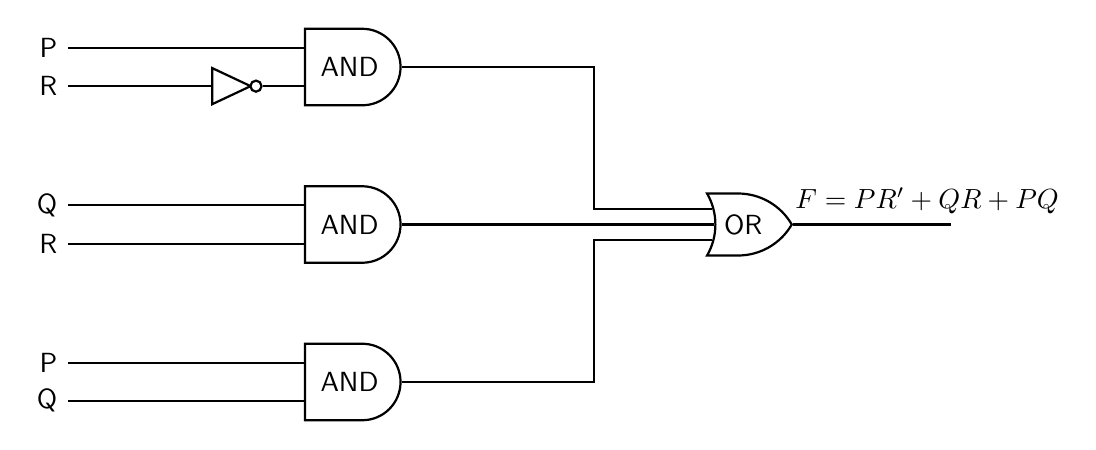
\begin{tikzpicture}[
        %Environment config
        font=\sffamily,
        thick,
        %Environment styles
        GateCfg/.style={
            logic gate inputs={normal,normal,normal},
            draw,
            scale=1
        }
    ]
    \path
        (0,0) node[and gate US,GateCfg](AND1){AND} 
            ++ (0,-2) node[and gate US,GateCfg](AND2){AND}
            ++ (0,-2) node[and gate US,GateCfg](AND3){AND}  
            ++ (5,2) node[or gate US,GateCfg](OR1){OR}
        (AND1.input 3)
            ++ (-1,0) node[not gate US, draw](N1){};

    \draw
        (OR1.input 1) -- ++(-1.5,0)node [midway,anchor=south]{} |- (AND1.output) 
        
        (OR1.input 2) -- ++(-1.5,0)node [midway,anchor=north]{} |- (AND2.output)
        
        (OR1.input 3) -- ++(-1.5,0)node [midway,anchor=north]{} |- (AND3.output)
        
        %(N2.output)--(AND2.input 3)
        
        (N1.output)--(AND1.input 3)
        
        %(N3.output)--(AND2.input 1)
        
        (AND1.input 1) 
            -- ++(-3,0) coordinate (init) node[anchor=east]{P}
            node[pos=0.6](temp){}
            
	  (AND2.input 1)
	  -- ++(-3,0) coordinate (init) node[anchor=east]{Q}
	  
	  (AND2.input 3)
	  -- ++(-3,0) coordinate (init) node[anchor=east]{R}
	  
	  (AND3.input 1)
	  -- ++(-3,0) coordinate (init) node[anchor=east]{P}
	  
	  (AND3.input 3)
	  -- ++(-3,0) coordinate (init) node[anchor=east]{Q}
            
       % (N1-| temp)
        %    ++(0,5pt) edge (temp.center)
        %    arc (90:-90:5pt) |- (N3.input)
            
            
        (init |- N1) node[anchor=east]{R} 
            -- (N1.input) node[pos=0.4](temp2){}
            
            
        %(temp2.center) |- (N2.input)
        
        
        (OR1.output) -- ++(2,0) node [midway,anchor=south]{$
        \qquad\qquad F = PR^{\prime} + QR + PQ$};
        
        
\end{tikzpicture} 
\end{center}


$$
F(P,Q,R) = QR + PR^{\prime} + PQ = \Sigma{m(3,4,6,7)}
$$

همانطور که در تابع جدید F مشاهده می شود، F دیگر SOP مینیمم نیست اما مشکل Hazard در آن برطرف شده است

جدول کارنو برای تابع F به صورت زیر می باشد :

\begin{center}
\begin{karnaugh-map}[4][2][1][$bc$][$a$]
\maxterms{0,1,2,5}
\minterms{3,4,6,7}
\implicantedge{4}{4}{6}{6}
\implicant{3}{7}
\implicant{7}{6}
\end{karnaugh-map}
\end{center}

در جدول کارنوی بالا مشاهده می شود که تمام زوج های 1 که با هم همسایه هستند پوشش داده شده اند و بنابراین از Hazard جلوگیری می شود

\newpage

\section{حذف static-0-hazard}

به طور مشابه برای حذف static-0-hazard به جای 1 ها 0 ها را در نظر می گیریم و نگاه میکنیم که کدام 0 های همسایه به عنوان گروه در نظر گرفته نشده اند که باعث static-0-hazard شده است\newline

راه حل حذف static-0-hazard مشابه حذف static-1-hazard می باشد فقط اینکه به جای SOP، باید POS برای نوشتن تابع در نظر گرفته شود


\section{Dynamic-Hazard}

Dynamic-Hazard مانند Static-Hazard می باشد که تغییر ورودی قبل از ثبات به حالت نهایی به صورت لحظه ای از 0 به 1 یا از 1 به 0 تغییر پیدا کند، اما در Dynamic-Hazard این اتفاق چندین بار و در زمان های مختلف رخ می دهد

ِDynamic-Hazard در مدار های پیچیده تر که مسیر های مختلف با تاخیرهای زمانی مختلف وجود دارد رخ می دهد


\begin{center}
	\includegraphics[scale=0.8]{./dynamic-hazards-1.jpg}
	%\caption{}
\end{center}

\subsection{حذف Dynamic-Hazard}

در صورتی که تمام Static-Hazard ها از یک مدار حذف شوند، Dynamic-Hazard اتفاق نخواهد افتاد

\end{document}